\newpage
\section{Utilisation}

Le menu permet d'accéder aux différentes possibilitées du site web.

\begin{figure}[H]
	\centering
	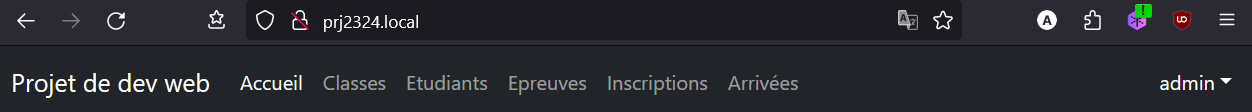
\includegraphics[keepaspectratio,width=15cm]{images/Emploi3}
	\caption{Navbar du site web}
\end{figure}

La structure pour les Classes, les Etudiants et les Epreuves est identiques. La page principal permet de visualiser la liste des éléments, de faire une recherche sur ceux-ci, d'accéder aux formulaire de création de l'élément et d'afficher les détails de ceux-ci :

\begin{enumerate}
	\item Permet d'effectuer une recherche d'un élément
	\item Permet d'accéder au formulaire de création de l'élement
	\item Permet d'afficher un élément, ce qui permet de voir / éditer / supprimer celui-ci
	\item Permet de naviguer parmit les éléments quand ceux-ci sont supérieur à 10.
\end{enumerate}

\begin{figure}[H]
	\centering
	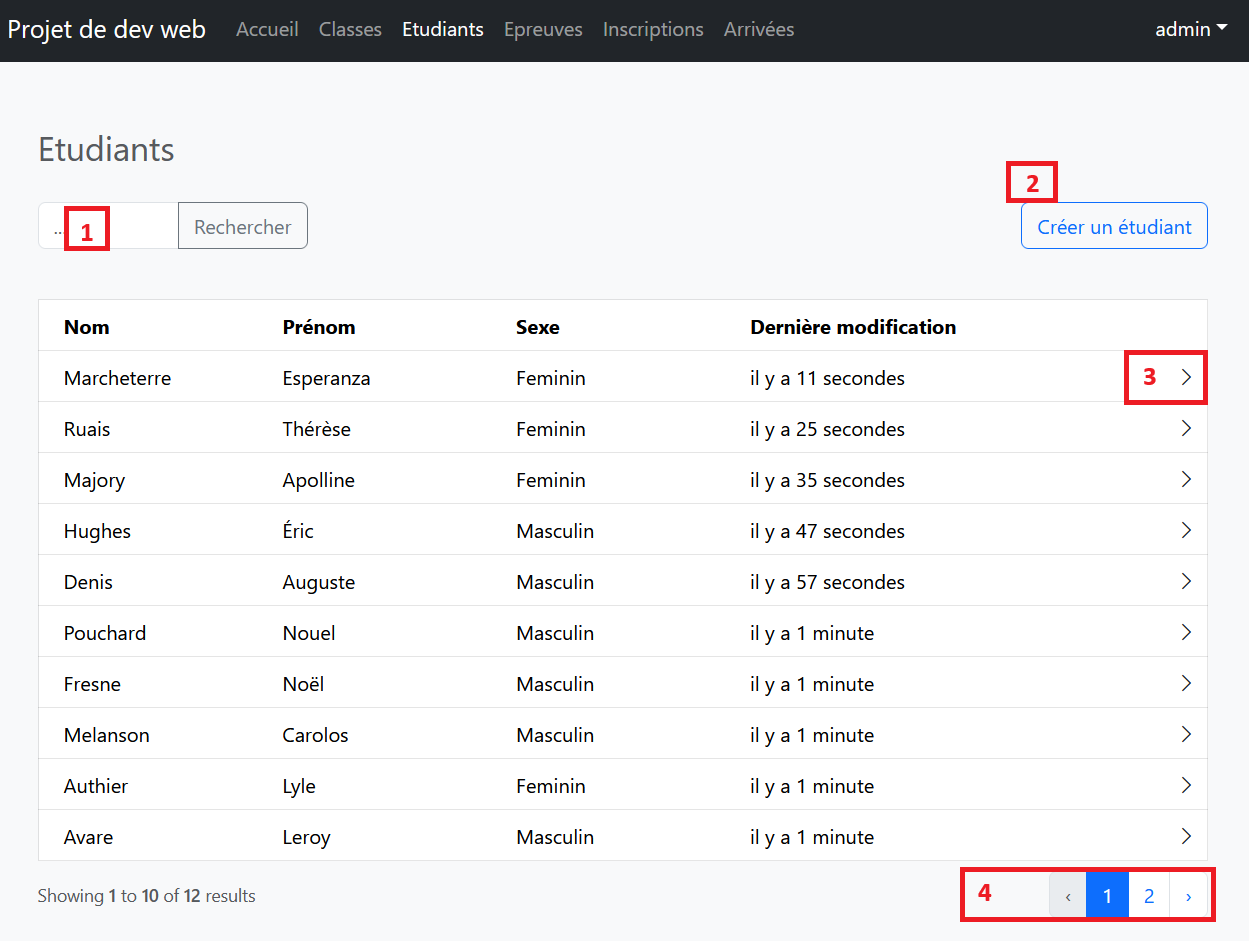
\includegraphics[keepaspectratio,width=12cm]{images/Emploi4}
	\caption{Page CRUD Etudiant}
\end{figure}

\newpage
Affichage de l'élément

\begin{enumerate}
	\item Zone d'affichage / d'édition de l'élément
	\item Accèder a la suppression de l'élément ( avec confirmation )
	\item Enregistre les modifications effectuée dans la zone d'édition
\end{enumerate}

\begin{figure}[H]
	\centering
	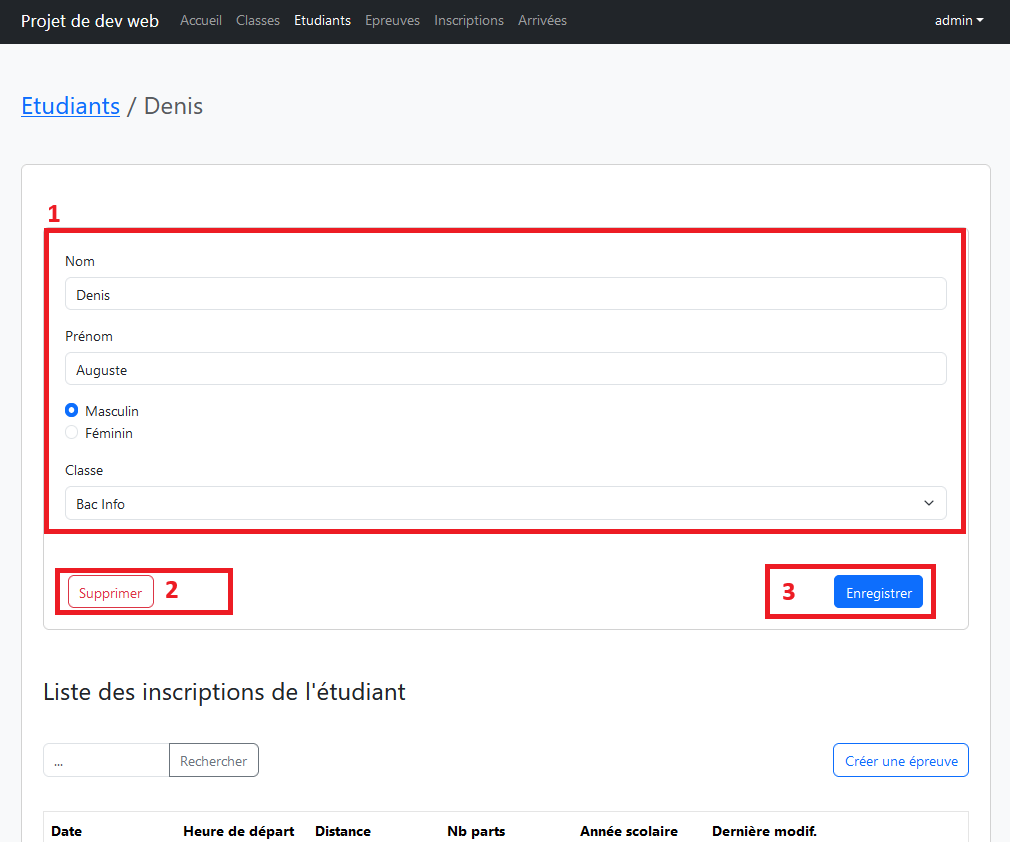
\includegraphics[keepaspectratio,width=12cm]{images/Emploi6}
	\caption{Formulaire création Etudiant}
\end{figure}


Pour les inscriptions, il nous faut selectionner l'épreuve qui nous interesse

\begin{figure}[H]
	\centering
	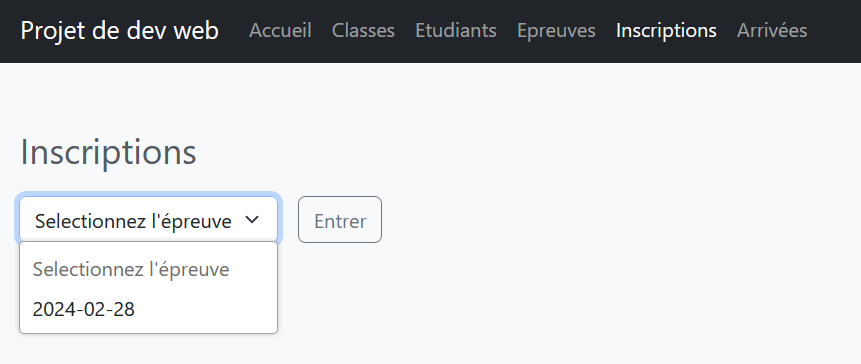
\includegraphics[keepaspectratio,width=12cm]{images/Emploi7}
	\caption{Formulaire de sélection d'une épreuve}
\end{figure}

\newpage
Nous sommes alors rediriger vers la page d'inscription, pour l'inscription il faut une heure (si pas encodé dans l'épreuve) et un type de coureur (run/walk) : Ensuite appuyé sur le + Vert afin de valider l'inscription.

\begin{figure}[H]
	\centering
	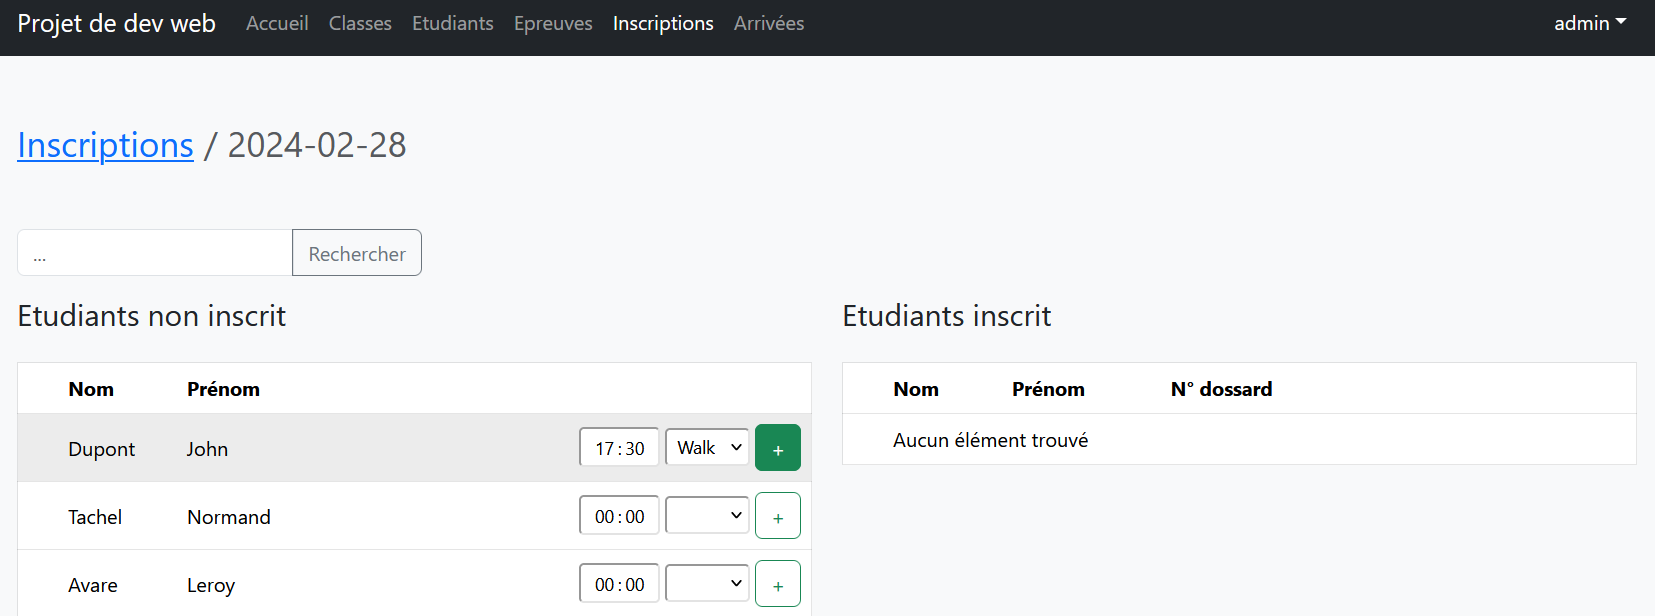
\includegraphics[keepaspectratio,width=12cm]{images/Emploi8}
	\caption{Formulaire d'inscription}
\end{figure}

L'étudiant devrait alors apparaitre dans la liste des étudiants inscrits

\begin{figure}[H]
	\centering
	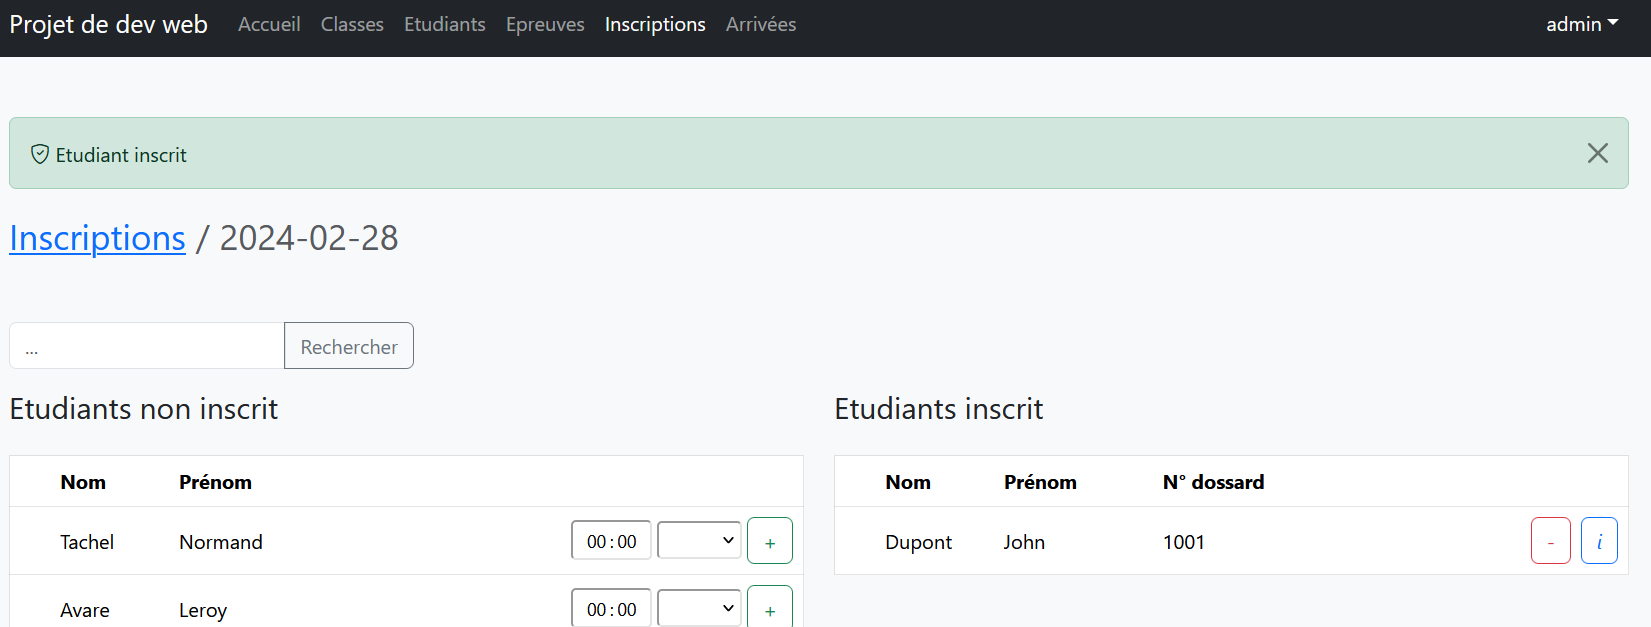
\includegraphics[keepaspectratio,width=12cm]{images/Emploi9}
	\caption{Formulaire d'inscription}
\end{figure}

\begin{itemize}[label=$\bullet$]
	\item Le '- Rouge' permet alors de désinscrire l'étudiant (uniquement si il n'a pas fini l'épreuve).
	\item Le 'i bleu' permet d'afficher et d'éditer (si l'épreuve n'est pas terminé) l'inscription.
\end{itemize}

Pour les arrivées, il nous faut selectionner l'épreuve qui nous interesse

\begin{figure}[H]
	\centering
	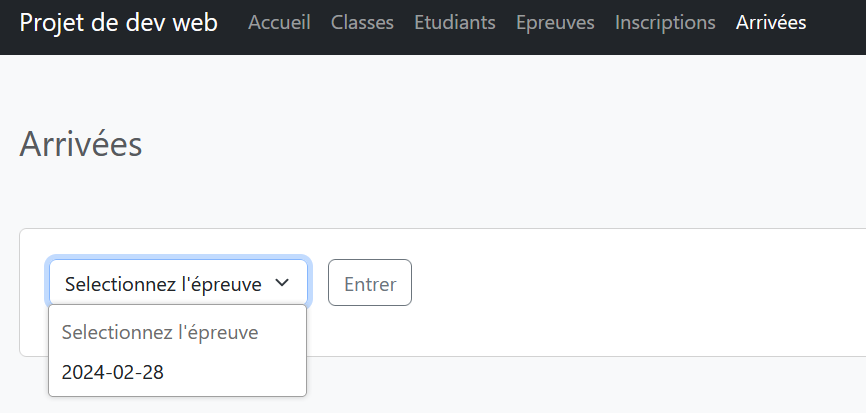
\includegraphics[keepaspectratio,width=12cm]{images/Emploi10}
	\caption{Formulaire de sélection d'une épreuve}
\end{figure}

Il faut encodé le n° de dossard (trouvable dans les tableaux d'inscriptions aux épreuves) et enregistré :

\begin{figure}[H]
	\centering
	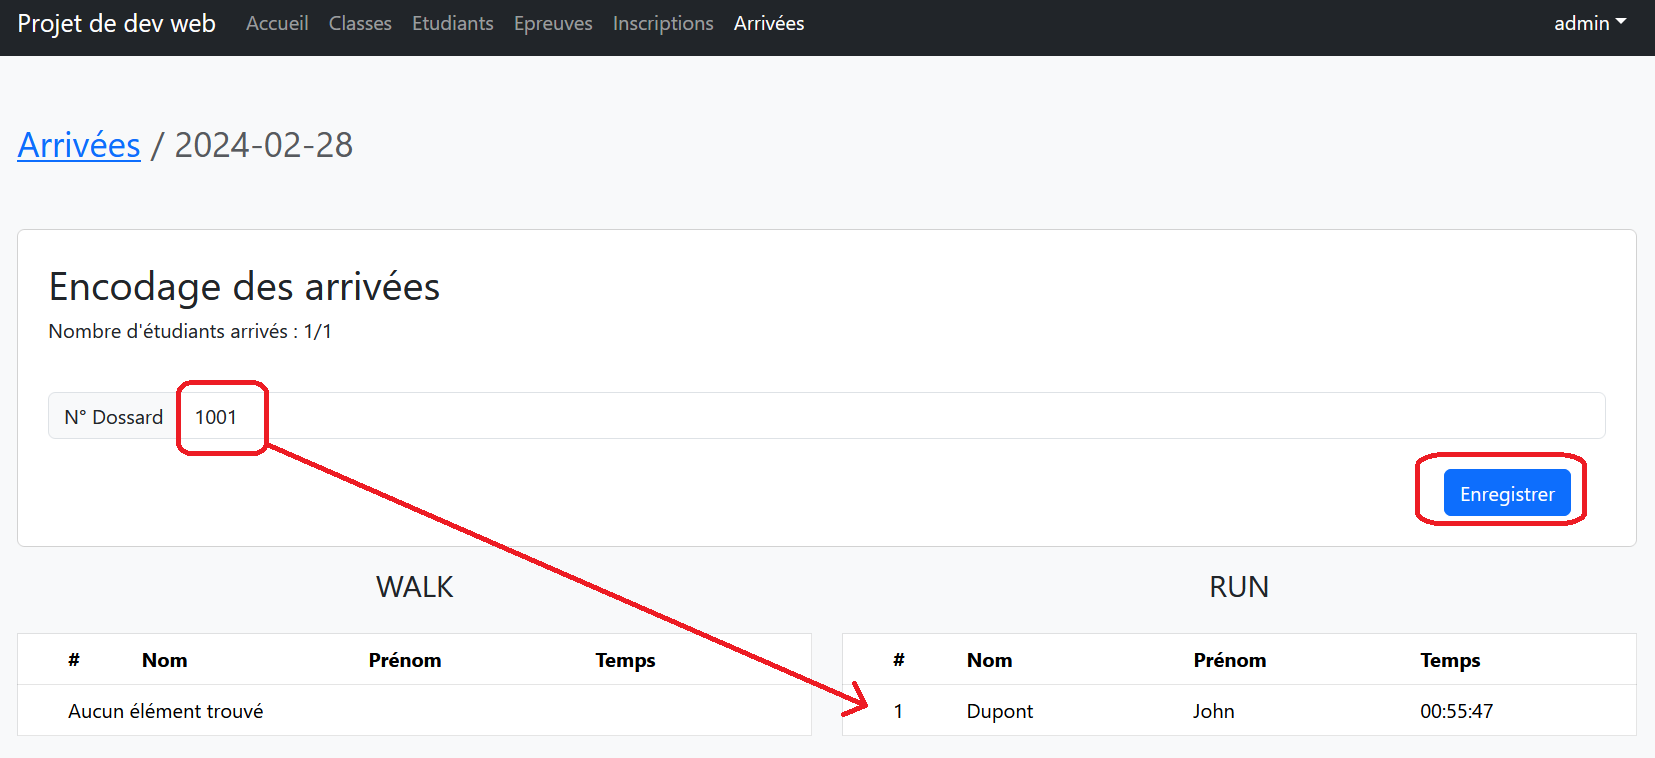
\includegraphics[keepaspectratio,width=12cm]{images/Emploi11}
	\caption{Formulaire d'encodage des arrivées}
\end{figure}